\subsection*{Objective}
As the Food-101 dataset mostly consisted of meals \parencite{food101}, it was decided to extend the
dataset slightly by including some single foods such as:
\begin{itemize}
    \item{cheese}
    \item{grapes}
    \item{banana}
    \item{apple}
    \item{orange}
    \item{spaghetti}
    \item{roll}
\end{itemize}

To collect these images, the ImageNet repository was utilised to search for
these foods individually and then download the subset of images to be included
with the Food 101 dataset \parencite{imagenet}.
This new extended dataset was named Food-101+.
The retrain.py script was run on the Food-101+ dataset as in
\ref{inception}.

\subsection*{Network Architecture}
The Inception V3 Model was used for this experiment.

\subsection*{Dataset}
In this experiment the Food-101+ dataset was used.

\subsection*{Libraries}
TensorFlow and NumPy are used in the retrain.py script.

\subsection*{Script}
As seen in \ref{extended}.

\subsection*{Results}
For this model, an accuracy of 55.3\% was achieved.

For example, an image of a banana (Figure \ref{fig:banana}) was fed into the model with
the following results:
\begin{itemize}
    \item{banana 0.9962}
    \item{orange 0.0009}
    \item{cheese 0.0003}
    \item{frozen yoghurt carpaccio 0.0002}
    \item{churros 0.0001}
\end{itemize}
 
\begin{figure}
\centering
    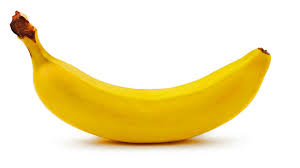
\includegraphics{banana}
    \caption{Banana - sourced from http://www.ciaoimports.com/}
    \label{fig:banana}
\end{figure}

\subsection*{Analysis}
The slight increase in accuracy in \ref{inception}, from 54.8\% to 55.3\%, makes
sense. Since the model was pre-trained using the ImageNet dataset and all the
new images used were from ImageNet, we would expect a higher classification
accuracy on the new additions to the dataset. This would overall increase the
average classification accuracy.
